% =============================================================
%  Maksim Privalov - CV (LaTeX)
%  Compile: pdflatex cv.tex   (needs photo.jpg in the same folder)
%  Works on Overleaf: upload cv.tex + photo.jpg, compiler pdfLaTeX
% =============================================================
\documentclass[10pt,a4paper]{article}

\usepackage[T1]{fontenc}
\usepackage[utf8]{inputenc}
\usepackage[scaled]{helvet}
\renewcommand{\familydefault}{\sfdefault}
\usepackage[a4paper,top=0.9cm,bottom=0.8cm,left=1.4cm,right=1.4cm]{geometry}
\usepackage{graphicx}
\usepackage{enumitem}
\usepackage{titlesec}
\usepackage{tabularx}
\usepackage[hidelinks]{hyperref}
\usepackage{xcolor}

\definecolor{linkblue}{HTML}{1155CC}
\newcommand{\link}[2]{\href{#1}{\textcolor{linkblue}{\underline{#2}}}}

\pagestyle{empty}
\setlength{\parindent}{0pt}
\setlength{\tabcolsep}{0pt}

% Section heading: centered title with a rule underneath
\titleformat{\section}{\large\bfseries\centering}{}{0pt}{}[\vspace{-6pt}\rule{\textwidth}{0.4pt}]
\titlespacing*{\section}{0pt}{4pt}{3pt}

\setlist[itemize]{leftmargin=1.4em,itemsep=0pt,topsep=1pt,parsep=0pt,label=\textbullet}

% \job{Organization}{Location}{Role}{Dates}
\newcommand{\job}[4]{%
  \textbf{#1}\hfill #2\\
  \underline{#3}\hfill #4\par}
% \edu{School, City}{Dates}{Degree}
\newcommand{\edu}[3]{%
  #1\hfill #2\\
  #3\par}

\begin{document}

% ------------------------- HEADER ----------------------------
\begin{minipage}[c]{0.15\textwidth}
  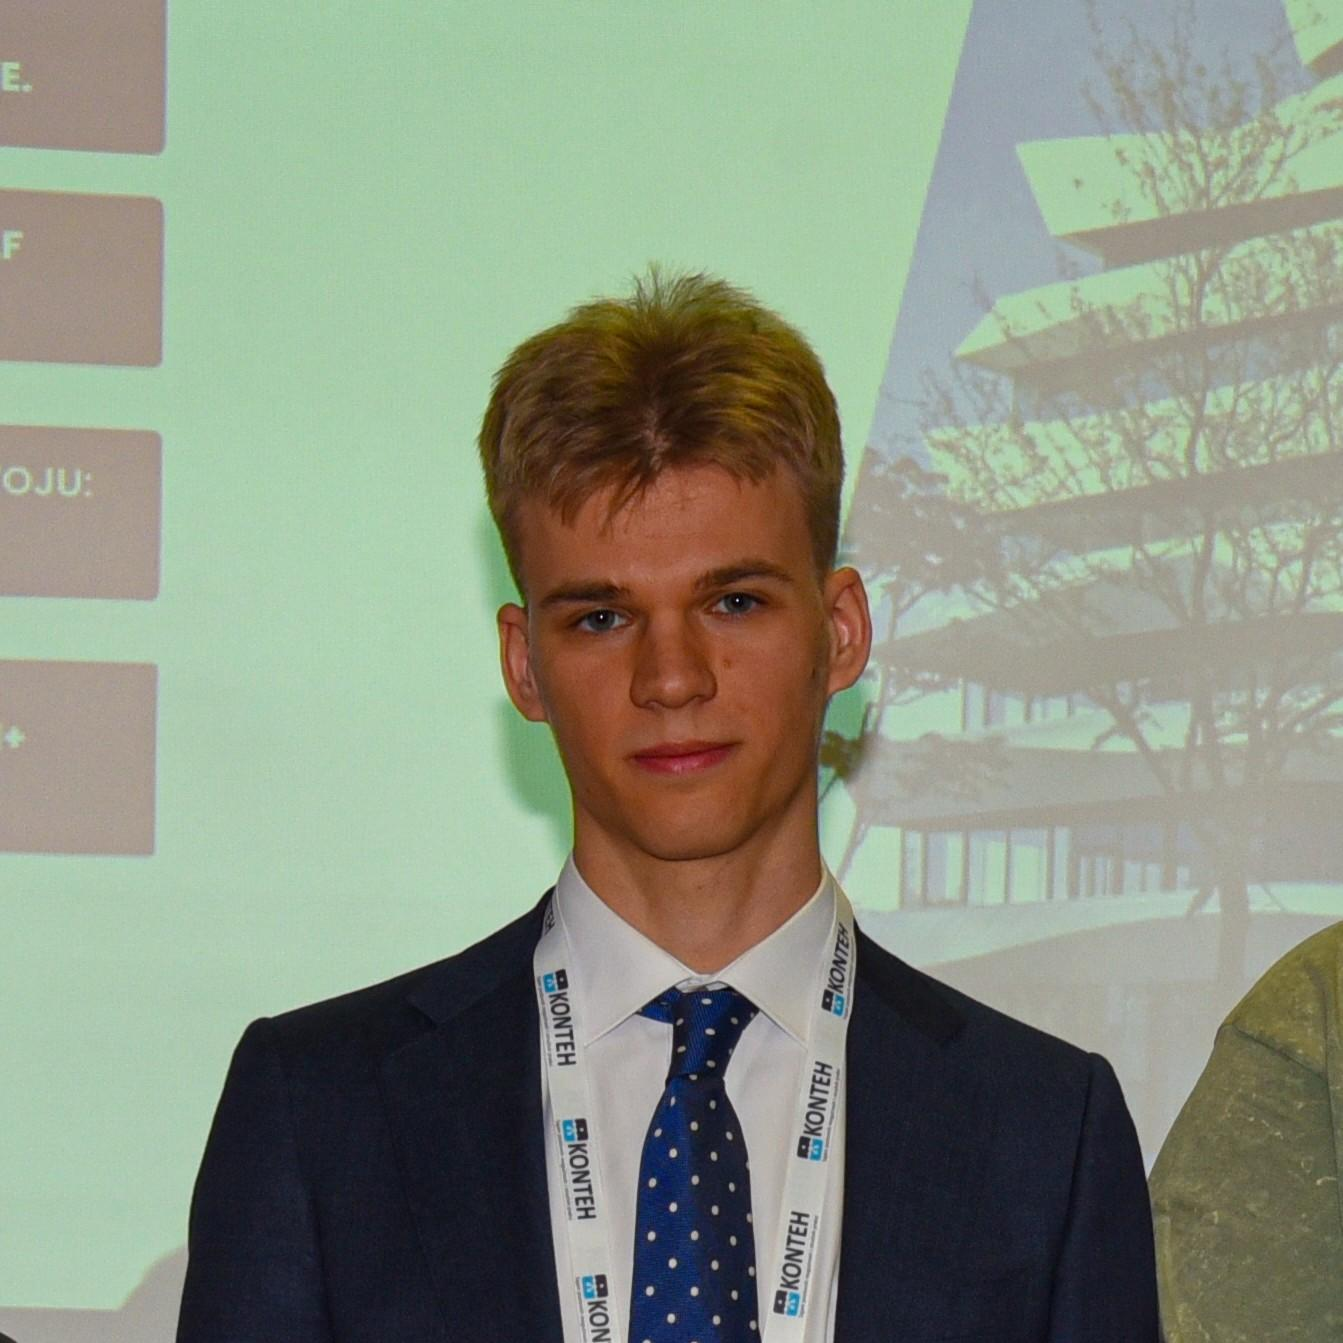
\includegraphics[width=\linewidth]{photo.jpg}
\end{minipage}%
\begin{minipage}[c]{0.70\textwidth}
  \centering
  {\LARGE\bfseries Maksim Privalov}\\[2pt]
  {\large Java Software Engineer}\\[2pt]
  \textit{Backend engineer with production experience in financial systems.}\\[2pt]
  +381-64-553-44-85 \,|\, \link{mailto:mprivalovs@gmail.com}{mprivalovs@gmail.com} \,|\, Novi Sad, Serbia\\[1pt]
\end{minipage}%
\hfill

% ------------------------- EXPERIENCE ------------------------
\section{Professional Experience}

\job{Faculty of Technical Sciences, University of Novi Sad}{Novi Sad, Serbia}{Software Engineer}{Mar 2026 -- Present}
\begin{itemize}
  \item Integrated embedded \textit{Apache Superset} dashboards into a Java desktop business system end to end; built a Spring Boot token
        service issuing short-lived guest tokens with row-level security derived from existing role-based permissions,
        enabling seamless sign-on without BI accounts or client-side credentials.
\item Designed and implemented a multi-tenant architecture with per-request configuration resolution for a platform serving
        50,000+ users, consolidating service instances into one and cutting server RAM usage by \textasciitilde86\%.
  \item Extended a Windows-only digital document signing system to support macOS and Linux by re-architecting
        the solution around \textit{Java PKCS\#11} libraries, eliminating client-side middleware and simplifying deployment.
  \item \textit{Technologies: Java, Spring Boot, Kafka, Redis, Prometheus, Grafana, Apache Superset, Microsoft SQL Server, Scrum.}
\end{itemize}

\vspace{3pt}
\job{Digital Access Logic}{Belgrade, Serbia}{Software Engineer}{Oct 2024 -- Apr 2025}
\begin{itemize}
  \item Integrated payment processing through \textit{a bank API broker} and implemented automated fiscal receipt
        generation to meet regulatory compliance requirements.
  \item Built a microservice-based ticketing system serving multiple clients in the entertainment industry, from
        design through production deployment.
  \item \textit{Technologies: Java, Spring Boot, PostgreSQL, OpenAPI, Postman, React, Scrum.}
\end{itemize}

\vspace{3pt}
\job{KONTEH}{Novi Sad, Serbia}{KONTEH 2026 Algorithmic Contest Organizer}{Dec 2025 -- Mar 2026}
\begin{itemize}
  \item Organized and ran a university-level algorithmic contest, sponsored by \textbf{Nordeus}; created problems,
        prepared test cases, set up the contest platform and defined the contest structure and rules.
\end{itemize}

% ------------------------- PROJECTS --------------------------
\section{Projects}
\begin{itemize}
  \item \link{https://github.com/maksimprivalov/payment-processing-service}{\textbf{Payment Processing Service}} (Rust, Axum, PostgreSQL, Docker) -- 6 microservices with saga orchestration,
        idempotent payments, double-entry ledger and audit log.
  \item \link{https://github.com/maksimprivalov/credit-card-fraud-detection}{\textbf{Fraud Detection System}} (Java, Spring Boot, Drools) -- real-time rule-based transaction scoring with
        complex event processing, hierarchical rules and explainable decisions.
  \item \textbf{Cloud Music App} (AWS Lambda, DynamoDB, S3, Cognito, Python, Angular) -- team-built serverless
        music streaming app with single-table DynamoDB design and stream-driven subscriber notifications.
  \item \textbf{CopyBot} (Java, Spring, Python/Flask, PostgreSQL, Docker, Selenium) -- commercialized Telegram bot for
        cross-posting between social networks, launched in 2024.
\end{itemize}

% ------------------------- SKILLS ----------------------------
\section{Skills}
\begin{tabularx}{\textwidth}{@{}l@{\hspace{6pt}}X@{}}
  \textbf{Languages:}        & Java, Kotlin, Rust, Python, SQL \;\textperiodcentered\; \textit{familiar:} Go, C++, C\#, TypeScript \\
  \textbf{Backend:}          & Spring Boot, Spring Security, Hibernate/JPA, Flyway, Axum, Drools, REST \\
  \textbf{Databases:}        & PostgreSQL, Microsoft SQL Server, Oracle, Redis, MongoDB, DynamoDB \\
  \textbf{Messaging:}        & Apache Kafka, RabbitMQ \\
  \textbf{Security:}         & OAuth 2.0, OpenID Connect, Keycloak, PKCS\#11, digital signatures \\
  \textbf{DevOps \& Cloud:}  & Docker, Kubernetes, AWS, Prometheus, Grafana, GitLab CI, Apache Superset, Git, Linux \\
  \textbf{Testing:}          & JUnit, Mockito, Postman \\
  \textbf{Practices:}        & Microservices, serverless, saga pattern, idempotency, double-entry ledger, SOLID \\
  \textbf{Methodologies:}    & Agile, Scrum, Kanban \;\textperiodcentered\; \textit{tools:} Trello, OpenProject, Miro \\
\end{tabularx}

% ------------------------- EDUCATION -------------------------
\section{Education \& Achievements}
\edu{\textbf{Faculty of Technical Sciences, University of Novi Sad}, Novi Sad, Serbia}{Oct 2026 -- Present}
    {Master of Software Engineering and Information Technologies, E-Business}
\vspace{3pt}
\edu{\textbf{Faculty of Technical Sciences, University of Novi Sad}, Novi Sad, Serbia}{Oct 2023 -- Sept 2026}
    {Bachelor of Software Engineering and Information Technologies \,\textperiodcentered\, GPA: 9 / 10}
\begin{itemize}
  \item Thesis: \textit{Application of OAuth and OpenID in microservice architecture}
\end{itemize}
\vspace{3pt}
\edu{\textbf{ITMO University}, Saint Petersburg, Russia}{Sept 2021 -- June 2023}
    {Bachelor of Neurotechnologies and Software Engineering \,\textperiodcentered\, GPA: B+ / A}
\vspace{3pt}
\textbf{Course:} MIT 15.S08 \textit{FinTech: Shaping the Financial World} (graduate level, MIT OCW)\par
\vspace{3pt}
\textbf{Phystech International 2020} medalist \hfill \textbf{Languages:} Serbian (fluent), Russian (native), English (C1)


\end{document}